\documentclass[12pt]{report}%{memoir}

\usepackage[utf8]{inputenc}
\usepackage[T1]{fontenc}
\usepackage[english]{babel}

\usepackage[a4paper]{geometry}  % Pour indiquer le format de page

% Pour la bibliographie
\usepackage[backend=biber,style=reading,sorting=nyvt]{biblatex}
\bibliography{Bibliographie}

\usepackage[style=french]{csquotes}

% Pour les liens
\usepackage{hyperref}
\hypersetup{
    colorlinks,
    citecolor=black,
    filecolor=black,
    linkcolor=black,
    urlcolor=blue
}

% Pour que les figures apparaissent sur la bonne page
\usepackage{float}

\usepackage{verbatim}

% Pour les annexes
\usepackage[toc,page]{appendix}

% Pour les images
\usepackage{graphicx}

%Multiple figures
\usepackage{subcaption}

\title{\textbf{LO53 Wi-Fi Positioning System\\ Lab report}}
\author{Thomas Gagneret\\ Stéphane Parunakian\\ Tao Sauvage}
\date{}

\begin{document}

\maketitle

\input{introduction.tex}

\setcounter{tocdepth}{1}
\tableofcontents

\chapter{Access Points}

The first main component of the Wi-Fi positioning system is the configuration
of the Access Points. In this chapter we describe how an AP works and how to
configure it.

\section{Linked list of the UEs}

First of all, the AP needs a data structure in order to save the different
measures of each User Equipment.

\subsection{Internal data structure}

Since UE measurements can be described as a simple structure containing only
two attributes -- the RSSI value and when this value has been retrieved -- its
seemed to be obvious to use a linked list.

\paragraph{}
The timer gives the AP the ability to delete a sample after a certain amount of
time which ensures to only keep accurate new values.

\paragraph{}
It becomes natural that the list is composed of elements where each of them
contains the MAC address of UE and a sample as shown below:

\begin{figure}[H]
  \centering
  \includegraphics[scale=.6]{./ap/ap_list.png}
  \caption{Simplified linked list that each AP uses.}
\end{figure}

\subsection{Keep it up-to-date}

In the previous section, we quickly presented the timer attribute of an UE
measurement. We now go deeper and show why this is important.

\paragraph{}
Since an UE is moving all the time -- walking, going from the door to the
window, etc. -- keeping its measurements for too long will distort its
localization.

\paragraph{}
Therefore, in order to ensure the best possible accuracy, each measurement has
a timer and as soon as it reaches a life-span higher than a second, it is
removed from the list.

\paragraph{}
It is possible to constantly remove the old measurements using a daemon thread
that checks the `deadline` attribute of a list element as shown below:

\begin{figure}[H]
  \centering
  \includegraphics[scale=.7]{./ap/ap_list_thread.png}
  \caption{Remove old measurements in the list.}
\end{figure}

Due to a lack of time, we were not able to complete the implementation of this
feature in our project.

\subsection{Build the response}

In order to prepare the communication between the AP and the Positioning
Server, the AP list also gives a function that will convert the list into a
JSON formatted response.

\paragraph{}
Named `build\_buffer`, this function looks for a specific MAC address in the
list. It then retrieves the RSSI values the AP has and computes their average
value.

\paragraph{}
Then, using the `snprintf` standard C function, it converts the result into a
JSON dictionary, fully prepared to be sent back to the PS.

\section{Passive Sniffer}

We have seen how the AP stores the data. Let us now see how it finds each
value.

\subsection{Listen to Wi-Fi packets}

In order to find the MAC addresses and the RSSI values of each device, it needs
to sniff the network for any Wi-Fi signals sent by the UEs. The AP achieves
this sniffing by using the \emph{PCAP} library.

\paragraph{}
It sets up a hook on its wireless interface in order to intercept any
Wi-Fi packets on the network like shown in the scenario below:

\begin{figure}[H]
  \centering
  \includegraphics[scale=.5]{./ap/mobile_with_aps.png}
  \caption{Each AP sniffs the Wi-Fi packets of the network.}
\end{figure}

\subsection{Extract the values}

Then for each packet, it extracts the MAC address and the RSSI value fields and
stores them into its list.

\begin{figure}[H]
  \centering
  \includegraphics[scale=.7]{./ap/focus_mobile_with_aps.png}
  \caption{For each packet, the AP extracts two fields.}
\end{figure}

\paragraph{}
For some times, we had a bug when using the \emph{PCAP} library. The sneakiest
problem we have met occurred because of the version the \emph{PCAP} library
that was running on the AP.

\paragraph{}
Indeed, for some versions, a field was added in the header and triggered a
buffer overflow when trying to retrieve the different informations we were
looking for.

\section{HTTP Daemon}

Last but not least, the AP needs a way to communicate with the PS. This section
describes how we manage to set up a communication system between both.

\paragraph{}
At this point, the AP is able the measure every RSSI values for any devices on
the network and stores them. It is also able to convert them to a JSON
formatted dictionary.

\paragraph{}
So in order to send that dictionary to the PS, we have set up a HTTP daemon
using the \emph{MicroHTTP} library.

\paragraph{}
When being fired up, it initializes that daemon using the
\emph{start\_microhttpd} function. As a callback function, the AP passes the
\emph{connection\_callback} one that reacts to any \emph{?mac=} HTTP requests.

\paragraph{}
Hence the AP is now able to communicate with the PS. The
\emph{connection\_callback} is triggered each time the server asks the
measurements of an UE. It then processes the list and builds the response.

\section{Run the program}

We now have every parts of the AP -- a data structure, a sniffer and a HTTP
daemon -- except how to configure and install it on the AP itself. This section
answers theses questions.

\subsection{Configuration}

The only configuration our project requires concerns the HTTP daemon and the
interface on which to set up the sniffer.

\paragraph{}
The \emph{http\_daemon.h} file defines two constants:

\begin{enumerate}
    \item The port on which the daemon will listen to. By
        default it is set to \emph{8080}
    \item The MAC address of the AP.
\end{enumerate}

\paragraph{}
Then the interface can be set up in the \emph{main.c} file.

\subsection{Installation}

Then, in order to create the program, we provide a \emph{Makefile} along with
the source files. Using the command \emph{make all} will generate the binary
(it requires the \emph{OpenWRT} toolchain).

\paragraph{}
Then the binary has to be copied onto the AP (using the \emph{scp} command for
instance).

\paragraph{}
Last, the command \emph{./ap\_daemon.bin} as to be run in order to run the
binary on the AP.


\chapter{Positioning server}

\paragraph{}
In this chapter, we will speak about the positioning server part of our project. 

    \section{Tools and versions}

\paragraph{}
Before seeing the server itself, lets see the different tools used for its
creation.

        \subsection{Java}

\paragraph{}
This server is coded in Java 7, the programming language of Oracle. So the
different servlets must use TomCat 7.

%        \subsection{Git}

        \subsection{Simulation scripts}

\paragraph{}
In order to test the server, without having to setup all the elements of the
project (Access points, mobile device), three Python scripts have been written:

\begin{description}
    \item [AccessPoint] Simulate the response of an access point.
    \item [MobileDevice (Calibration)] Simulate the calibration request of a
        mobile device.
    \item [MobileDevice (Localisation)] Simulate the localisation request of a
        mobile device.
\end{description}

    \section{Programm}

\paragraph{}
Now we will look at the server.

        \subsection{DAO}

\paragraph{}
A major element of the server code is the Data Access Object (DAO). It is the
link between the database and the code. It allows the programm to manipulate
data as it was objects, without having to care about the database. The DAO
creates objects from information in the database, and updates information in the
database from objects.

\paragraph{}
The major advantage of this concept is the possibility to change the way to
store data easily. Only the DAO interface needs to be modified in case we want,
for example, to use a NoSQL database.

        \subsection{Calibration}

\paragraph{}
The Calibration servlet is called by mobile devices to put calibration information
in the server database.

\paragraph{}
How the servlet works:
\begin{enumerate}
    \item A mobile device send a calibration request, with a map id and
        coordinates.
    \item The servlet get a list of all routers present in database.
    \item If there is enough routers, it goes on, else it stops.
    \item It sends RSSI requests to router and wait no more than 500 ms for the
        response.
    \item If there is enough useful responses, it stores them in the database
        (RSSI table), else it stops.
    \item It sends a response to the mobile device.
\end{enumerate}

        \subsection{Localisation}

\paragraph{}
The Localisation servlet is called by mobile devices who want their
localisation.

\paragraph{}
How the servlet works:
\begin{enumerate}
    \item A mobile device send a localisation request, with no parameters.
    \item The servlet get a list of all routers present in the database.
    \item If there is enough routers, it goes on, else it stops.
    \item It sends RSSI requests to router and wait no more than 500 ms for the
        response.
    \item If there is enough useful responses, it stores them in the database
        (TempRSSI table), else it stops.
    \item It gets every location calibrated from the database and calculate the
        distance with the data in the TempRSSI table, for each location.
    \item It returns the closest location to the mobile device (map id,
        coordinates).
\end{enumerate}


    \subsection{Computation of a location}

\paragraph{}
The two servlets uses the same function for calculating the RSSI distance. This
function is used to compute the distance between the new location and all the
known locations. During a localisation request, the nearest point is calculated
and returned to the mobile device.

    \section{Database}

\paragraph{}
The database of the server is shared between the servlets. Its structure is
almost the same as in the subject. There is only one addition: an ``ip'' column
in the AccessPoints table (it is more reliable than using the id for the last
part of the ip).

\begin{figure}[h]
  \centering
  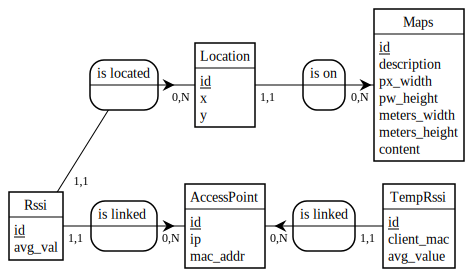
\includegraphics[scale=1]{./positioning_server/db.pdf}
  \caption{Database}
\end{figure}

        \subsection{Creation script}

\paragraph{}
In order to create the database, a postgresql script has been created. It
creates a user ``lo53'' with a password ``lo53'' and a database ``lo53\_rssi''.

        \subsection{Filling}

\paragraph{}
The filing of the database has to be handmade, except for the Maps table. As
this table contains binary data, it is quite difficult to do it manually. So we
wrote a filling script to do this. This script put maps pictures in the
database, and get informations about maps from text files like this one :

\verbatiminput{./positioning_server/pic.txt}

\paragraph{}
The size in pixel of the picture is automatically determined, thank to the PIL
library. The addition in the database uses the psycopg2 connector.

    \section{Configuration file}

\paragraph{}
Some values of the positioning server may need adjustments. These values should
not be hardcoded, because it is not practical at all. So the servlets share a
configuration file named \emph{config.properties}. Below is the content of this
file.

\verbatiminput{./positioning_server/config.properties}

\paragraph{}
This file already exists, and can be found in the WEB-INF/classes folder of the
positioning server. Without it, servlets won't be able to work correctly.

\paragraph{}
Here is the explanation for each value of this file :
\begin{description}
    \item[url, user and password] These values are used to configure database
        information.
    \item[ap\_port] It is used for the communication between servlets and access
        points. We assume that all access points use the same port.
    \item[ap\_timeout] It indicates how long must servlets wait for access points
        responses during RSSI requests.
    \item[min\_ap] It represents the minimum number of access points needed in
        order to make a RSSI request. If there is not enough router, no request
        will be made.
    \item[min\_samples] The minimum number of RSSI samples by access point
        required.
    \item[min\_measurements] The minimum number of temporary RSSI measurements
        needed in order to calculate a RSSI distance or validating the RSSI
        measurements for a location.
\end{description}


\chapter{Android}
In this chapter we will talk about the two applications used by the different users to communicate with the server.

\section{Settings}
First, for this two applications we designed a preference activity which allows the user to change different values to access the server. Indeed the address, the port and the servlet to use can be changed.

\begin{figure}[h!]
  	\centering
    \includegraphics[scale=0.1]{./android/Settings.png}
  \caption{Settings activity}
\end{figure}


\section{Setup Tool}
Now, we will talk about the setup tool application which allows a network administrator for example to set some calibration points in the building. On the next figure you can see the different phase to use this application.


\begin{figure}[h]
        \centering
        \begin{subfigure}[b]{0.3\textwidth}
    			\includegraphics[scale=0.1]{./android/Setup_list.png}
                \caption{Choose your map}
                \label{fig:map_list}
        \end{subfigure}
        \begin{subfigure}[b]{0.3\textwidth}
                \includegraphics[scale=0.1]{./android/Setup_set.png}
                \caption{Display the map}
                \label{fig:map_set}
        \end{subfigure}
        \begin{subfigure}[b]{0.3\textwidth}
                \includegraphics[scale=0.1]{./android/Setup.png}
                \caption{Set calibration point}
                \label{fig:map}
        \end{subfigure}
        \caption{Setup Tools application}\label{fig:setup}
\end{figure}

\begin{itemize}
\item First, when you launch the application there is a list of all map available on the server which is displayed. It contains the id, a description and the size of the map in meters. Then you just have to select the correct one. It is also possible, when you know the id of the map to use the search bar. Indeed you just have to put the correct id and it will display the map just like if you choose it from the list. (See Figure \ref{fig:map_list})
\item Then when the map is displayed you have to click on the "set" button to be able to add a calibration point. (See Figure \ref{fig:map_set})
\item Once you clicked on the "set" button you can set your calibration point and click on "measure" to send all the information to the server. It's also possible to cancel using the "cancel" button which remove your calibration point (on the map). (See Figure \ref{fig:setup})
\end{itemize}

\section{Positioning}
Now we will talk about the positioning application which allow a user to be located in a building according to the calibration points set with the previous application.

\begin{figure}[h!]
  	\centering
    \includegraphics[scale=0.1]{./android/Positioning.png}
  \caption{Positioning application}
\end{figure}

This application is very simple. The user just have to click on "Start locating" and the application sends a positioning request to the server and display the result on the screen (map to display, position).


\section{RSSI values}

For this two applications the access points require a maximum of RSSI values. If the mobile does not communicate, the access points do not retrieve RSSI values which prevents the applications to work correctly. So in both application we ping the server but also launch a wifi scan which allow the access points to retrieve about 50 RSSI values.



\input{./conclusion.tex}

%\nocite{*}

%\printbibliography[heading=bibintoc]

\newpage
\thispagestyle{empty}
\null
\vspace{\fill}
\begin{center}
    \includegraphics[width=1in]{./license.png} \\
    This report is licensed under a Creative Commons Attribution 4.0
    International License.
\end{center}


\end{document}
